\begin{frame}[fragile]{Experimental Support for Modified Ping-Pong}
\begin{tikzpicture}[scaleall=1.0]
\pcuad{\textwidth}{\textheight}
%\showcuad
\path(nw) ++(-0.25,-0.4) node(plot)[graphics,anchor=north west]{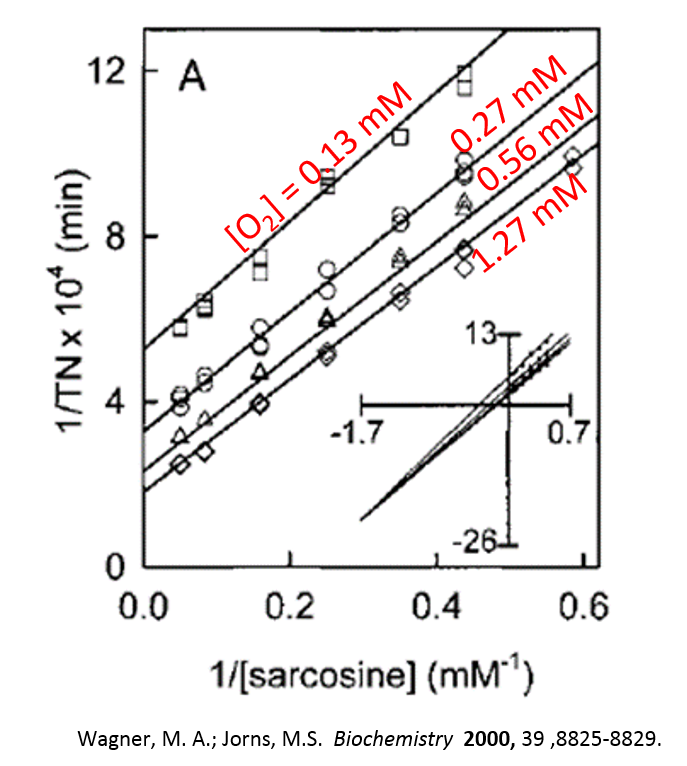
\includegraphics[width=0.6\textwidth]{msox_jorns_expt}}
          ++(6.5,-0.0) node(text) [shape=rectangle,anchor=north west,text width=0.4\textwidth] {
          Lineweaver-Burk slope-dependence on [O$_{\sf 2}$] indicates [O$_{\sf 2}$] and [S$_{\sf R}$] are not independent, suggesting \textcolor{red}{MPP}.}
          ++(0.0,-3.0) node(moretext) [shape=rectangle,anchor=north west,text width=0.4\textwidth]{
          \textcolor{green!80!black}{\bf Hypothesis:} MPP implies kinetics of O$_{\sf 2}$ entry and exit should be 
          sensitive to whether or not substrate is bound.  Test using simulations!};

\end{tikzpicture}
\end{frame}
